\section{Représentation de la vitesse (4 points)}

\begin{questions}
	\question Représenter la vitesse d'un objet à un instant précis, dans les conditions suivantes  :
	
	\begin{parts}
		\part[2] \begin{itemize}
			\item Mouvement : horizontal de gauche à droite;
			\item Valeur de la vitesse : 25 m/s;
			\item \'Echelle choisie: 1 cm pour 10 m/s.
			
		\end{itemize}
	
%		\makeemptybox{4cm}
		
		
		\part[2] \begin{itemize}
			\item Mouvement : chute verticale d'un objet;
			\item Valeur de la vitesse : 10 m/s;
			\item \'Echelle choisie: 1 cm pour 5 m/s.
		\end{itemize}
			
		
%		\makeemptybox{4cm}
	\end{parts}

%	\question[2] \'A l'aide d'un logiciel de traitement de vidéos, on peut repérer les positions successives prises par un point d'une grande roue lors de son mouvement.
%	
%	Sans tenir compte sa valeur, représenter la vitesse aux positions 3, 12, 22 et 33.
%	
%	\begin{center}
%		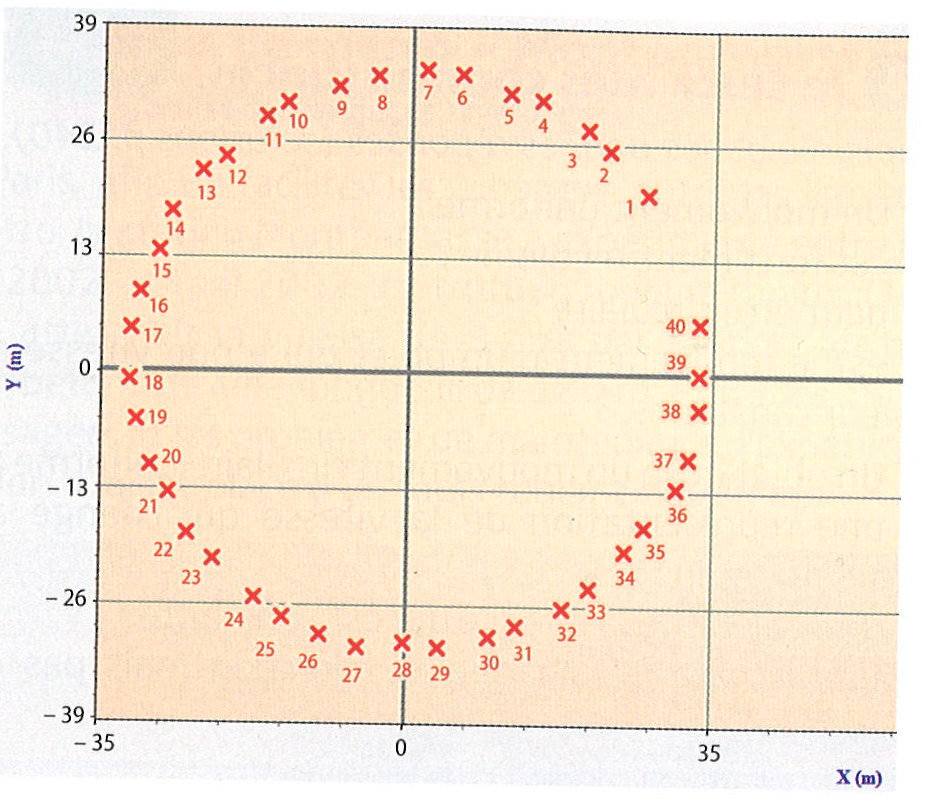
\includegraphics[scale=0.35]{roue}
%	\end{center}
\end{questions}